\documentclass[a4paper]{article} % a4paper option recommended
\usepackage[english]{babel}
\usepackage{uureport}
\usepackage{cite}
\usepackage{hyperref}
\usepackage{pgfplots}
\usepackage{float}
\usepackage{listings}
\usepackage{graphicx}
\usepackage{amsmath}
\bibliographystyle{alpha}


\title{Diplomacy}
\type{Report}
\course{Games \& Agents}

\author{A. Berland, B. Reigersberg, E. Koens, \\J. de Groot, K. van Katwijk, T. de Goeij}

\begin{document}
\maketitle
\tableofcontents
\newpage

\section{Introduction}
Diplomacy is an online multiplayer game based on the board game invented in 1954 by Allan B. Calhamer. The online version of the game has 137966 subscribed players, it can however be played by bots as well. A few bots have already been implemented, so far the best bot on the market is Albert. All these bots lack one common property, which is the ability to asses the other players. Therefore we tried to implement an Artificial Intelligent bot for this game, which is able to comprehend the actions of other bots and players. Our bot can deduce the best possible moves which are based on his own ideas and knowledge, he will also concern his current belief on the other player or bot. We made quite some progress and we will elaborate on our development of this bot in this paper.

\subsection{Diplomacy}
The online diplomacy game is based on the map of 1901 Europe, but can also be played on other maps. The map consists of three different nodes. These are divided in land provinces, coastal provinces and sea nodes.
\\The goal of the game is to be the first to hold more than half of the supply centers. Supply centers can be divided in two types, Home Supply Centers and other Supply Centers (there is no actual difference in the game it self but we made the difference for the weight \& gains system). All Supply Centers sustain the military units, however only Home Supply Centers can build new units. In order to build new units a player has to own more Supply Centers than units this is done in the Build phase (Winter).
\\There are five phases in Diplomacy, as stated earlier there is the Build phase, which is called Winter in game. There are two Order phases (Summer and Fall) in which the player decides where to move his available units. After each order phase there is a retreat phase (Spring and Autumn). In the retreat phase any attacked units are forced to retreat. If there is no possible place to retreat to the unit needs to be disbanded (removed from the game).
\\The game revolves around two different type of units. On one side there is the Army unit type which moves on coastal and land provinces. The other unit type is the Fleet, this unit can move through coastal provinces and trough oceans. The Fleets can convoy Army units over the sea to other provinces. The armies all have the same power, so in order to take a province a player needs support moves.
\\The units have five types of moves. The first move is the HOLD move. With this move the unit stays on his current territory and therefore defend it.
Then there is the MOVE action, with it the unit moves from one province to an adjacent province.
Then there are two types of support moves, the SUPPORT HOLD, this is a support for the defending HOLD move. The SUPPORT HOLD gives the defending army an additional unit to defend with. And then there is the SUPPORT MOVE, which is basically the same but for attacking. The last move is the CONVOY move, for this move a player needs a fleet and an army. The fleet needs to be in the ocean. Then the army moves via the fleet over the ocean to the next province.
The CONVOY move can also be chained if mutiple fleets are adjacent, this is still seen as one move.

\section{Trust}


A very important underlying assumption in Diplomacy is that the initial relations with everyone is hostile. In other words, you have no reason to expect other players to leave your supply centers be as they have a strong incentive to claim them. Knowing that another power will not attack you is a tremendous benefit for a player as armies and fleets can be directed on offense against someone else while not being concerned about leaving supply centers adjacent to a pacifist power undefended. Below we have made some definitions of the implicit meaning of treaties based on the norms of the game.
\begin{description}
\item[Peace treaty]: Simply means that you will refrain from attacking each other.

\item[Alliance treaty]: Includes peace, but also imply an obligation to support each other in attacking a specific enemy.
\end{description}

Communication in Diplomacy offers cheap talk, an aspect of game theory which is defined as being costless due to not requiring players to sacrifice any resources exchanging words. However, one of the clinchers of the game itself lies within the complexity of deception - how would you ever trust the current treaty you have just made with a neighboring power? It is common knowledge for most Diplomacy players that there is a real incentive to exploit others when they have lowered their guard. Hence, one of the real talents of being a good player is to be able to take precautions, or in other words - recognize players who are likely to defect.

As trust is defined by keeping your end of a deal, it is impossible for two fully trustworthy players left in the game to ever finish if they are at peace. One possible solution to this problem is to explicitly state your peace/alliance proposals with a duration variable, expressed in game phases. An honest player will then be able to attack another honest player after the expiration of the peace treaty. However, due to the limitations of the DAIDE server in which our bot communicates with, there is no option to state a time constraint to any treaty, nor is this a norm by human players.

However, in most cases backstabbing a player whom you recently made a peace or alliance treaty with is judged as bigger breach of trust than someone who backstabs you after several phases after the treaty. After all, all treaties will cease to exist at some point, and this is common knowledge among all players of Diplomacy due to the winning conditions of the game. As such we have reached a more fuzzy alternative, implying that treaties decays ($D$) over time [CITATION ]. The reason why exponential is more fitting than linear is the fact that it should never fully dissolve, as there is no time constraint expressed in the treaty. We now have a way to decrement someone's trust  more dynamically when they choose to defect a treaty, respecting the norms of the game where the severity of defecting decreases over time. In addition, we need a constant rate of increment ($\tau$) as long as treaties are upheld which is essential to ever build up trust with anyone.\

For defecting a treaty: 
$T'_p = T_p - \frac{D^{-t}} {10}$ \\
\
For maintaining a treaty: 
$T'_p = T_p + (\tau \cdot t)$
\\
 \begin{center}
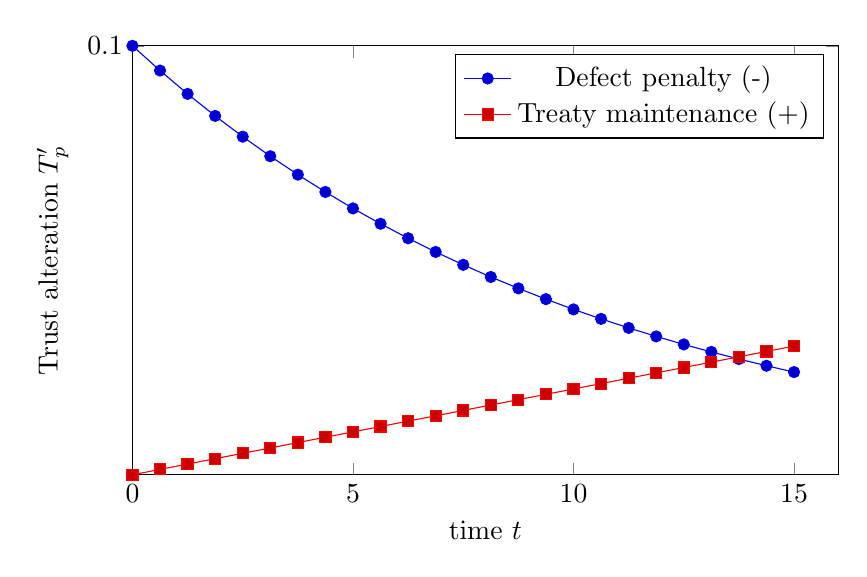
\begin{tikzpicture}
  \begin{axis}[ 
  	width = 300,
    height = 200,
    xlabel= time $t$,
    ylabel={Trust alteration $T'_p$},
    xtick = {0,5,10,15},
    ytick = {0.1},
    xmin = 0,
    ymin = 0,
    xmax = 16,
    ymax = 0.1,
    domain = 0:15
  ] 
    \addplot {(1.1^(-x)/10};
    \addplot {0.002*x};
    \legend{Defect penalty (-), Treaty maintenance (+)};
  \end{axis}
\end{tikzpicture}
\end{center}

It is crucial to understand that the trust-value assigned to different players in our system is not an indicator of how reliable they are. A player could for example reject a peace proposal and reliably not attack you consistently. But due to our expectations of the norms of peace, we expect no player nor bot to have this behavior. As such, in our system we choose to implement 'trust' as a fitness for choosing whom we should ally ourselves with, in addition to guiding how paranoid we should be against every other power. Having peace with someone you do not trust should be possible, but internally the bot should be paranoid in regards to defending his borders. The justification for such a possibility is for the untrusted power to have a chance to redeem itself if it chooses to adopt a more cooperative strategy. Given the decay of treaties, we can safely assume that the closer they are to diminishing, the more paranoid we should be. To repeat the inital statement of this section regarding seeing every power we do not have any treaty with as hostile, we assign them all with a full level of paranoia ($P = 1$). Every treaty initializes with an paranoia equal to the relevant powers current trust. 

  \[ P_p = \left\{ 
  \begin{array}{l l}
    1 - \Big( D^{-t} \cdot T_p \Big) & \quad \text{for $T > 0$} \\
 	1 & \quad \text{for $T = 0$}
    
  \end{array} \right.\]
  
  \begin{center}
\begin{tikzpicture}
  \begin{axis}[ 
  	width = 300,
    height = 200,
    xlabel= time $t$,
    ylabel={Paranoia $P_p$},
    xtick = {0,5,10,15},
    ytick = {1},
    xmin = 0,
    ymin = 0,
    xmax = 15,
    ymax = 1,
    domain = 0:15
  ] 
    \addplot {1-((1.1^(-x))*(0.8))};

  \end{axis}
\end{tikzpicture}
\end{center}


Paranoia [0-1]  is a value attached to any power within an instance of a game which offers us the ability to predict whether or not we should expect them to defect. A procedure to reduce paranoia of any power we already have a treaty with is to re-iterate the initial proposal. In practice it is equivalent to ask our ally 'is our deal still on?'. To attend the issue regarding a deadlock of two fully righteous powers who never wishes to break a treaty, one will eventually ask if the deal is still on in which the other is at liberty to decline. As a result, this solution to breaking peace/alliance is possible without breaching any trust.


Support obligations of alliances

Within a conjoint alliance treaty together with power A, there lies an agreement to conduct both defensive and offensive support moves against power B. However, considering the fact that there can only be one winner of power B’s supply centers, the alliance can only be mutually beneficial if both parties divide the spoils of war. However, there might be possible moves towards gaining a supply center given the accessibility of one's own units if they were not requested somewhere else by our ally. If one would ignore how other players viewed us (righteousness of 0), it would be rational to reject this request. This, however, is not a fair deal for the other party, as it can be exploited if it mindlessly helps the other with supports without realizing the other does not reciprocate. A solution is needed which makes us sensitive to injustice in terms of our spoils and our ally's spoils.

 In addition we also have a model of appropriate conduct if we would want to be righteous, implying that we would be permissible if the other party declined supporting us if we knew we were in debt - that is, knowing he has currently been supporting us more than he has received from us. But even if our personality is exploitive, we should also recognize those powers who are vulnerable to be exploited, namely altruists.

The function essentially captures the underlying obligation for allies to reciprocate support-moves. If a power asks for support all the time without reciprocating, its trust will decrement per support they reject when they owe us support. Given the fact that trust-values are altered online, the support-favor is stored as an attachment for every power per game.

An indirect consequence of this leaves exploiting players to be forced to team up with a high paranoia, which is a severe disadvantage compared to the cooperative players.

As we have now covered the trust mechanics, the remaining personality factor is that of trust initialization for new players our bot meets. A value of 0 implies that its fully cautious at the start of treaties, whereas 10 implies full naivety of opponents exploitative capabilities. 

A summary of trust increments and decrements for each treaty per phase:

Incrementation:
+ For every phase a treaty is maintained 
+ If you get support from an ally you consider altruistic

Decrementation: 
- Defect in upholding a treaty (backstab)
- If you get a rejection in your support proposal from an ally which you deem exploitive.


\
\


supIntolerance = $S$ 0.0005\\
time = $t$ \\
$D$ = 1.1 \\
$\tau$ = 0.002\\




  \[ T'_p = T_p + \left\{ 
  \begin{array}{l l}
    (S \cdot \sigma_p)^2 & \quad \text{if $\sigma_p > 0$ \& ACCEPT}\\
    -(S \cdot \sigma_p)^2 & \quad \text{if $\sigma_p < 0$ \& REJECT}\\
    \text{0} & \quad \text{if ($\sigma_p \le 0$ \& ACCEPT) or ($\sigma_p \geq 0$ \& REJECT)}
    
  \end{array} \right.\]
  \\
  
 \begin{center}
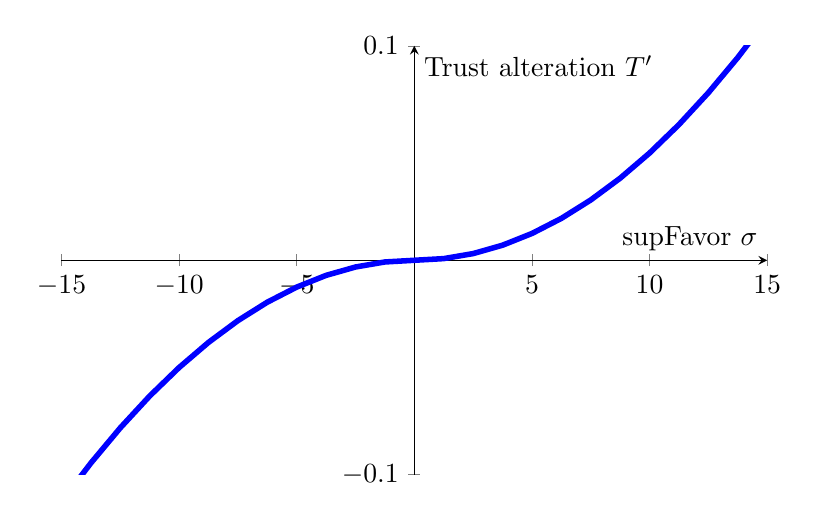
\begin{tikzpicture}
  \begin{axis}[ 
  	width = 300,
    height = 200,
  	axis x line = middle,
    axis y line = middle,
    xlabel= supFavor $\sigma$,
    ylabel={Trust alteration $T'$},
    xtick = {-15,-10,-5,0,5,10,15},
    ytick = {-0.1,0,0.1},
    xmin = -15,
    ymin = -0.1,
    xmax = 15,
    ymax = 0.1,
    domain = -15:15
  ] 
    \addplot [blue] [line width=2pt] {(x/abs(x))*((0.0005*x^2)};
  \end{axis}
\end{tikzpicture}
\end{center}

\section{Gain system}


In order for our AI to know where it should move it's units to, we make use of a gain system. For every province we calculate a gain value. This value signifies the importance of this province based on a variety of properties and heuristics. We weigh this gain with factors such as likeliness to succeed and whether we defect allies by moving to this province. 

\subsection{Gains}  

For each province the gain value signifies the importance of that province. To calculated the gain, we have selected a number of properties which we believe makes a province important (But can very easily be extended and adjusted). We divided these into four categories. 

\begin{itemize}
\item Supply gain
\item Defend gain
\item Counter gain
\item Kill gain
\end{itemize}

\subsubsection{Supply gain}

The supply gain is given to provinces which contain a supply center. In order to win the game one has to control more than half of all the supply centers. Also, the number of supply centers you control determines how much units you are allowed to have. Therefore, capturing supply centers is crucial to winning the game and these provinces are important and we give these a gain. There are however different types of supply centers we have to consider. 

Supply centers can be controlled by a power. If a supply center is not controlled by us (so either neutral or under control by any other power), we can potentially take over this supply center. We give these a gain $g_{supply}$. Supply centers we control have no real gain as we can not take them over again. However, in the case that there is nothing more important to do, we would prefer units to move to one of our supply centers as a means of defence. We therefore give a small symbolic gain $g_{ourSupply}$ to supply centers we own. 

Some supply centers are home supply centers. These are home to a specific power and a power can only build new units on his home supply centers. Additional to the importance of normal supply centers, capturing a home supply center from a power effectively disables this power from building new units there. Therefore we give these a different (higher) gain $g_{home}$. We only do this when this home supply center is under control by the corresponding power. If this is not the case, then this power is already blocked from building units there and there is no additional gain from taking this. In this case we treat is as a normal supply center and give gain $g_{supply}$.

Following this rule, our own home supply centers are also very important. As with normal supply centers, if we control them they get a small gain $g_{ourHome}$. However, if a home supply center is under control by another power it is very important to get it back in order to build new units. In this we assign a very high gain $g_{takenHome}$. 

\subsubsection{Defend gain}

Without defending the supply centers we already control, they will just as easy be taken back from us. The defend gain is therefore given to supply centers we control and are under threat. In order to do this we first have to quantify threat. We calculate the threat by a weighted sum of the first and second order enemies from the same power (e.g. the enemies one tile away and the enemies two tiles away respectively). 

$$threat = max_{threat_j}\{ threat_j : C_1 \sum_{i} e^{1}_{ij} + C_2 \sum_{i} e^{2}_{ij}\}$$

We have chosen to give the supply center a defend gain $g_{defend}$ if $threat > \varepsilon_{threat}$. As we belief that defending home supply centers is more important these get a different gain $g_{defendHome}$. 

\subsubsection{Counter gain}
Using only the aforementioned gains, we perceived that units on threatened home supply centers displaying  ``camping'' behaviour. The unit keeps defending the home supply center from a neighbouring enemy whereas the neighbouring is interested in the home supply center and hence does not move away. We therefore introduced a high counter gain $g_{counter}$, to provinces adjacent to a home supply center and containing an enemy unit. This way, instead of endlessly holding the home supply center, units will start to make offensive moves against adjacent enemies driving the threat away instead of waiting for it to go.        

\subsubsection{Kill gain}
Another thing we also witnessed by watching our AI play is that very often units of a power are on the far side of the map - far from any support. This units are often left unattended as a single unit is not considered a threat. We therefore introduced a kill gain $g_{kill}$. This is a very high gain for a province containing a lonely enemy unit (no other enemy units as close as two tiles away), and this unit has limited provinces $< \varepsilon_{kill}$ to retreat to - likely causing it to disband when attacked. 
Another issue solved by this, is that very often the last living unit of a power is left unattended and sometimes even regains considerable power. 

\subsection{Smoothing gains}


\subsubsection{Gain values}

We chose this gain because blablabla. This one should then be higher because bla. Therefore bla. Blip bloop blababliebloopie. 

\begin{figure}[H]
\centering
\begin{tabular}{| l | c |}
  \hline            
  {\bf Gain} & {\bf Value}\\
  {Supply Gains} &  \\
  $g_{supply}$ & 3.0 \\
  $g_{ourSupply}$ & 0.25 \\
  $g_{home}$ & 3.2 \\
  $g_{ourHome}$ & 0.3 \\
  $g_{takenHome}$ & 5.0 \\
  {Defend gains} &  \\
  $g_{defend}$ &  3.0 \\
  $g_{defendHome}$ & 3.2 \\
  {Counter gain} & \\
  $g_{counter}$ & 5.5 \\
  {Kill gain} & \\
  $g_{kill}$ & 5.0 \\
  \hline  
\end{tabular}
\caption{Values choses for the various gain variables}
\end{figure}


\section{Implementation}
\subsection{User manual}

\subsubsection{AIServer}
In order to run our AI, you first need an AIServer which runs the game and to which the AI can connect. In order for our AI to fully function we use the AIServer that can be downloaded from: 

\begin{sloppypar}
\noindent\url{http://johnnewbury.me.uk/diplomacy/downloads/aiserver/aiserver-0.38~1.1-release-notice.htm}
\end{sloppypar}

The AIServer contains a Windows executable file but also runs perfectly under Wine on Linux. Upon running this executable the user is presented with various options. For our AI, make sure that the \textit{Log All Messages} option is on and the press level is set to a minimum of 20 (otherwise the server does not allow for alliance negotiation). A new game can now be started by clicking the \textit{New Game} button. This opens up a lobby, and the game will start as soon as 7 players have joined.     

\subsubsection{DodoAI}
In order to compile and run the Java code you can either import it an Java IDE such as Eclipse or use the command line. For the latter option we have included a makefile in the $src$ directory. Make sure a Java SDK (OpenJDK or Sun) is installed. After a succesfull compilation (ignore the warnings) you can run the program by running the DodoAI class with Java. Assuming a Unix-like operating system:       
\begin{lstlisting}[frame=single] 
cd location/of/repository/src/
make
java ai.dodo.DodoAI [ip] [port] [options]
\end{lstlisting}

Where \textit{ip} should be the ip address of the server - if run locally on the same machine use \textit{localhost} for this. \textit{port} is the port on which the server is listening. The default option for this is 16713 but can be adjusted in the AIServer settings. After these two arguments, several options can be set with flags

\begin{description}
\item[-n [name]] Using the -n flag the name for the AI (default DodoAI) can be changed. 
\item[-l [filename]] Using the -l flag, you can set the location of the server log file. Using this log file the AI will extract the names of all AI's and corresponding power from the server log file. Though this is not allowed by official Daide rules, this allows our AI to know who plays which power during the game. This is necessary as one of our goals was to include reputation in our AI. Note that this option is only possible if the server runs on the same machine or has remote access to the server log file.  
\item[-f [filename]] The -f flag can be used to set a personality file for this AI in order to create a unique personality. An example of a personality file can be found somewhere TODO. Note that the personality file includes a name which will override a name given a name with the -n flag.  %TODO!!%.  
\item[-k] If the -k flag is given, the AI will require a keypress in order to submit it's orders at the end of a turn. This is very useful when observing an AI-only game, the game is over so fast that is impossible to see what happened. We recommend running a single instance of DodoAI with the -k flag (Instead of all 7), as the rest of the AI's will automatically have to wait for this instance.  
\end{description} 

\subsubsection{AIMapper}
In order to visualize the game or play against our AI yourself, you need the AIMapper. This AIMapper can be downloaded from: 

\begin{sloppypar}
\noindent\url{http://johnnewbury.me.uk/diplomacy/downloads/aimapper/aimapper-0.41~1.1-release-notice.htm}
\end{sloppypar}

As with the AIServer the AIMapper comes as a windows executable, but is fully functional under Wine in Linux. You can join as either an observer (only watch the game) or player (play yourself). 


\subsection{Support}

In order to prepare a movement, it is important to know whether the movement can be effective. Consider the situation where a province is occupied by one enemy unit, then it is useless to try to move to that province with only one unit. In this case at least two units are needed to kick the enemy out, and perheps additional units are needed to cope with enemy support. The gain system calculates the amount of units that is needed to invade a province. This is done by keeping track of all units that possibly can support each province, as well for the own power as for the enemy powers. At least one unit is needed when a province is not occupied by an enemy unit, and at least two units are needed for a occupied province. For each possibly supporting enemy unit, a unit from the own power has maybe to support. But it is not certain whether this unit needs to support, since it is not possible to know on forehand whether the enemy unit will support. To cope with this uncertainty, we incorparated a risk variable. This variable determines how large the support needs to be. It could become possible to move to an unoccupied province with only one unit and without any further support, while the enemy has two potentially supporting units. For each of the units that can support, a check is done whether a random value is larger than $\alpha_{sup}$ and the number of support is increased by one when this evaluates true. However this does not determine which units need to support, only how much units need to support in the case that this province is going to be invaded. We have chosen to define $\alpha_{sup}$ as $risk^{k}$ where risk is between 0 and 1, and k is the amount of enemy support and $k>0$. By the amount of enemy support is meant the highest enemy support of all individual enemies. We choose for an exponential function since we believe that when something is important and hard, it is better to strike hard. Besides a human experiences a move whith too less units as a stupid move. 

\subsubsection{Drawback support}
Consider the case that all units already have a task assigned, except for one unit. This unit could move to an unoccupied province surrounded by three enemy units. Since the enemy support is quitte high, it is likely that there also will be a high number support assigned to this province. As result this province is filtered out as untakeable. But how realistic is this? Since it concerns the last unit, the priority of the province won't be very high and therefore it is not likely that the enemy would use so much units on this province. To cope with this drawback, the risk variable should be slightly increased every time a target is chosen. In this way very low risks are taken with high priority targets, and more risk is taken with lower priority targets. 

\subsection{Threat}

\subsection{Movement Phase} 

During the movement phase the units get orders assigned to defend or invade provinces, or to support another units. There are countless possibilities of how units can be deployed, and by far not enough computational power to consider each option.   

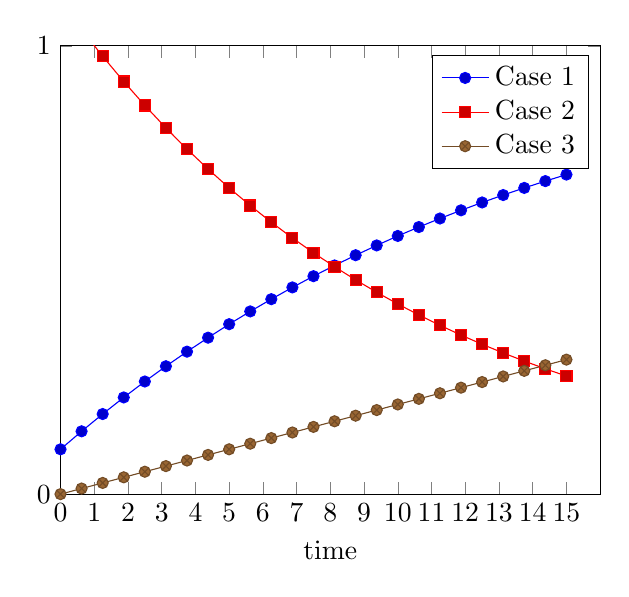
\begin{tikzpicture}
  \begin{axis}[ 
    xlabel= time,
    ylabel={},
    xtick = {0,1,2,3,4,5,6,7,8,9,10,11,12,13,14,15},
    ytick = {0,1},
    xmin = 0,
    ymin = 0,
    xmax = 16,
    ymax = 1,
    domain = 0:15
  ] 
    \addplot {1-((1.1^(-x))*(0.9+0.02*x))};
    \addplot {(1.1^(1-x))};
    \addplot {0.02*x};
    \legend{Case 1,Case 2, Case 3};
  \end{axis}
\end{tikzpicture}

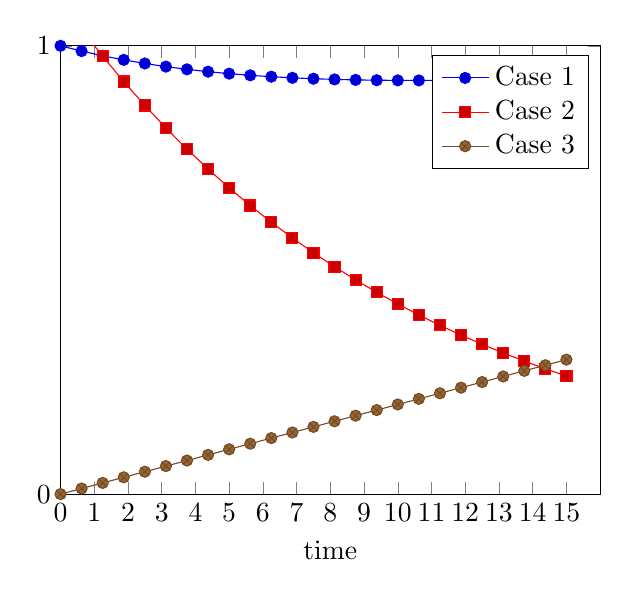
\begin{tikzpicture}
  \begin{axis}[ 
    xlabel= time,
    ylabel={},
    xtick = {0,1,2,3,4,5,6,7,8,9,10,11,12,13,14,15},
    ytick = {0,1},
    xmin = 0,
    ymin = 0,
    xmax = 16,
    ymax = 1,
    domain = 0:15
  ] 
    \addplot {1-((1.1^(-x))*(0.0+0.02*x))};
    \addplot {(1.1^(1-x))};
    \addplot {0.02*x};
    \legend{Case 1,Case 2, Case 3};
  \end{axis}
\end{tikzpicture}


% \begin{thebibliography}{1}

%   \bibitem{notes} Pacheco, J.M., Santos, F.C., Souza, M.O. and Skyrms, B., {\em Evolutionary dynamics of collective action in N-person stag hunt dilemmas}  2009.

%   \bibitem{impj}  da Costa Ferreira, A.F., {\em DipBlue: a Diplomacy Agent with Strategic and Trust Reasoning} For Jury Evaluation.

% \end{thebibliography}

\bibliography{references}{}

\end{document}